\documentclass[tikz,border=3.14pt]{standalone}
\usepackage{tikz}
\usetikzlibrary{arrows.meta}
\usepackage{amsmath}
\usepackage{physics}

\ExplSyntaxOn
\msg_redirect_name:nnn { siunitx } { physics-pkg } { none }
\ExplSyntaxOff

\begin{document}
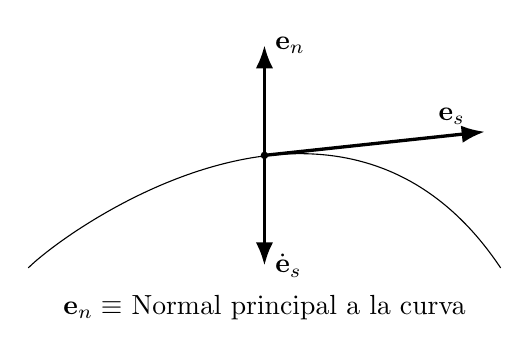
\begin{tikzpicture}[scale=2,
		vector/.style={-{Latex}, very thick}]

        \draw (0, 0) .. controls (0.25, 0.25) and (2, 1.5) .. (3, 0);
 
        \draw [fill] (1.5, 0.715) circle (0.02);
        \draw [vector] (1.5, 0.715) -- ++(1.4, 0.15) node [pos=0.85, above] {$\vb{e}_{s}$};

        \draw [vector] (1.5, 0.715) -- ++(0, 0.7) node [right, pos=1] {$\vb{e}_{n}$};
        \draw [vector] (1.5, 0.715) -- ++(0, -0.7) node [right, pos=1] {$\dot{\vb{e}}_{s}$};

        \node at (1.5, -0.25) {$\vb{e}_{n} \equiv $ Normal principal a la curva};

\end{tikzpicture}
\end{document}